\chapter{Sprint 2 --- Matching and Scoring Engine}
\chaptermark{Sprint 2 --- Matching \& Scoring}
\label{chap:sprint-2}

This chapter presents the realization of Sprint 2: turning Sprint 1's
trustworthy extraction into the project's core value, a ranked,
sub-scored candidate shortlist per TDR position, covering the sprint's
backlog, design, implementation, testing, and review.

\section{Sprint Goal}

\begin{quote}
Given a TDR position and the CV pool, produce a real ranked shortlist
with sub-scores, visible in a working matching results view.
\end{quote}

Sprint 2 ran July 13--17, 2026, with 42 points committed. Unlike Sprint 1
(which had to prove a single high-risk integration), this sprint's risk
was distributed across a genuine pipeline of five sequential stages
(coarse retrieval, skill normalization, hard filtering, soft scoring,
persistence/render), each depending on the last: correctness had to
hold at every stage for the ranked list at the end to mean anything.

\section{Sprint Backlog}

Table~\ref{tab:sprint2-backlog} lists Sprint 2's committed stories, points, and status.

\begin{table}[H]
  \centering
  \caption{Sprint 2 backlog}
  \label{tab:sprint2-backlog}
  \begin{tabular}{@{}p{1.7cm}p{11.2cm}p{1.3cm}p{2.7cm}@{}}
    \toprule
    ID & Story & Points & Status \\
    \midrule
    ADQ-10 & Build the reference skill/certification taxonomy (seed data) & 5 & Done \\
    ADQ-11 & Cheap pre-filter: shortlist plausible candidates before detailed scoring & 5 & Done \\
    ADQ-12 & Match raw skill terms to the taxonomy via embeddings & 8 & Done \\
    ADQ-13 & Add a reranking pass to improve skill-matching accuracy & 3 & Done \\
    ADQ-14 & Retry unmatched skill terms via a translation/abbreviation lookup & 5 & Done \\
    ADQ-15 & Scoring: hard eligibility filters (diploma, experience, certifications) & 3 & Done \\
    ADQ-16 & Scoring: weighted skill/sector sub-scores & 5 & Done \\
    ADQ-17 & Matching results page (demoable slice) & 5 & Done \\
    ADQ-18 & First retrieval-quality metrics against a hand-labeled gold set & 3 & Done \\
    \bottomrule
  \end{tabular}
\end{table}

All 42 points shipped within the sprint window. The scoring step's
LLM-judgment and historical-decision memory calibration were deferred to
Sprint 3 (ADQ-19) from the start, as planned: Sprint 2's scoring is
deliberately rules-and-embeddings only, with zero LLM calls anywhere in
the matching path.

Beyond the committed backlog, two further rounds of work happened that
weren't separate backlog items but were essential to the sprint actually
being trustworthy: growing the candidate pool, TDR sample, and skill
taxonomy well past what the company provided (covered in Implementation,
Section~\ref{sec:s2-impl}), and, once the matching view was demoable, a
code-review pass plus two rounds of live-testing-driven fixes (covered in
Testing, Section~\ref{sec:s2-testing}).

\section{Analysis}

The sprint goal reduces to one new user-facing flow on top of Sprint 1's
upload screens: given an already-extracted TDR, produce and display a
ranked list of candidates per expert position. The same actor from
Sprint 1 drives it:

\begin{description}
  \item[HR / bid manager] clicks \emph{Run matching} on an extracted TDR,
    then reviews the ranked shortlist per position: compatibility
    score, pass/fail hard-filter status with a reason, and skill/sector
    sub-scores.
\end{description}

The matching pipeline itself shortlists plausible candidates cheaply
before doing any expensive per-candidate work, normalizes both the
position's and each candidate's raw skill strings against a shared
taxonomy, applies hard eligibility filters, computes weighted soft
scores for whoever's left, and persists and serves the ranked result.

One use case was in scope: \emph{Run Matching for a TDR}, decomposing
into \emph{View Ranked Shortlist} per position once results land. Report
generation with cited rationale, anomaly detection, and human-in-the-loop
review/override are explicitly out of scope, needing the LLM reasoning
layer deferred to Sprint 3.

The central non-functional constraint this sprint: matching has to stay
cheap enough to run against the whole CV pool per TDR position without
either an LLM call or an unindexed full-table scan being the bottleneck.
This shaped the two-phase architecture described in Design
(Section~\ref{sec:s2-design}): a cheap embedding-only coarse filter runs
before any of the more expensive per-candidate normalization or scoring
work.

\section{Design}
\label{sec:s2-design}

Three diagrams cover this sprint's design: the use cases it adds on top
of Sprint 1's, the key classes the matching pipeline introduces, and the
sequence one matching run actually follows end to end.

\subsection{Use Case Diagram}

Figure~\ref{fig:s2-usecase} shows this sprint's use cases, extending
Sprint 1's upload/preview flows: \emph{Run Matching} requires a TDR
whose extraction has already completed (\texttt{status = "done"});
attempting it earlier is rejected with a 409 by
\texttt{TdrsService.run\_matching}, reusing the same
\texttt{ResourceNotReadyError} pattern Sprint 1 established for
in-progress extractions.

\begin{figure}[H]
  \centering
  
\includegraphics[width=0.5\textwidth]{s2-usecase.png}
  \caption[Sprint 2 use case diagram]{Sprint 2 use case diagram: running a match and viewing its
  ranked shortlist.}
  \label{fig:s2-usecase}
\end{figure}

\subsection{Class Diagram (key classes)}

Figure~\ref{fig:s2-class} shows the sprint's key classes.
\texttt{NormalizedSkill} (\texttt{app/domain/matching.py}) is a raw term
matched, or not, to a taxonomy canonical id, with a confidence and a
\texttt{matched\_via} label; \texttt{SubScores} carries only skill and
sector this sprint, deliberately left \texttt{null} rather than faked
until a real computation exists for education, experience,
certification, and language;
\texttt{MatchResult} is the persisted hard-filter outcome, failure
reasons, compatibility score, and sub-scores. Coarse retrieval
(\texttt{app/features/matching/coarse\_retrieval.py},
\texttt{shortlist\_candidates}) and the pipeline nodes
(\texttt{app/features/pipeline/nodes/\{normalize\_skills,score\}.py})
operate on these classes but are functions, not shown as boxes below.

\begin{figure}[H]
  \centering
  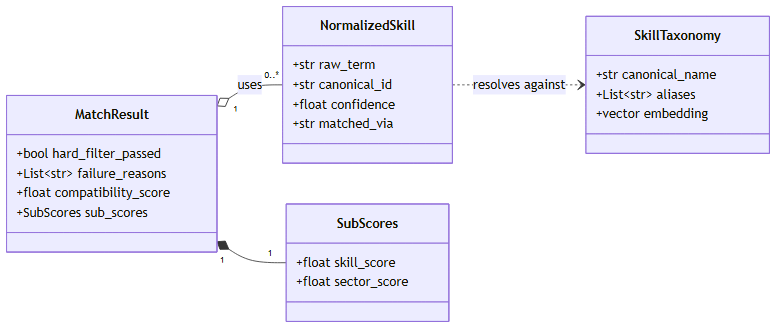
\includegraphics[width=0.65\textwidth]{s2-class.png}
  \caption[Sprint 2 class diagram]{Sprint 2 key classes: skill normalization and match scoring.}
  \label{fig:s2-class}
\end{figure}

\subsection{Sequence: Run Matching}

Figure~\ref{fig:s2-sequence} traces one matching run: the request
returns immediately (202) while an RQ worker
(\texttt{app/worker/matching\_tasks.py}) does the work, shortlisting
candidates per position (top $\sim$30 by cosine similarity, re-ranked
by sector/years boost, final shortlist $\sim$10), normalizing the
position's own skills and sector once (candidate-independent, computed
before the per-candidate loop), then normalizing, filtering, and scoring
each shortlisted candidate before replacing that position's stale
results in one transaction, so reruns stay idempotent.

\begin{figure}[H]
  \centering
  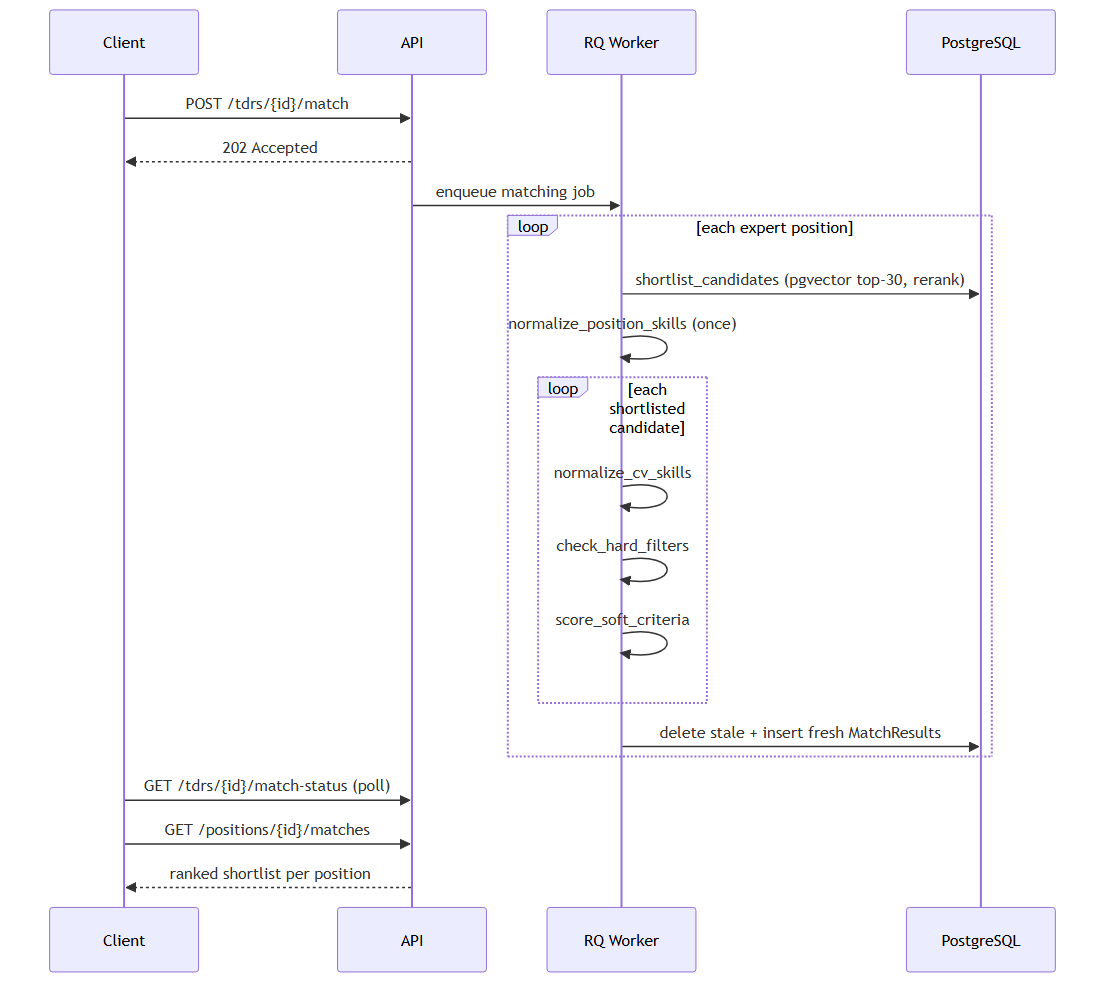
\includegraphics[width=0.7\textwidth]{s2-sequence.png}
  \caption[Sprint 2 matching sequence]{Sprint 2 sequence: asynchronous matching, per-position
  shortlisting, and per-candidate scoring.}
  \label{fig:s2-sequence}
\end{figure}

\section{Implementation}
\label{sec:s2-impl}

Each backlog story is covered in the order the pipeline actually runs
them, from the taxonomy they all depend on through to the two rounds of
work the team took on beyond the original backlog.

\subsection{ADQ-10: Skill/certification taxonomy}

\texttt{backend/app/features/pipeline/seed\_data/skill\_taxonomy.json} +
\texttt{backend/scripts/seed\_skill\_taxonomy.py} (idempotent, upserts by
canonical name). Started at 70 hand-curated terms against the Sprint 1
sample data; grown to 104 later in the sprint (Data ownership,
Section~\ref{sec:s2-data-ownership}) by mining vocabulary directly out of
a much larger real TDR sample.

\subsection{ADQ-11: Coarse retrieval}

Before any expensive per-candidate work, every candidate is ranked
cheaply by embedding similarity alone:

\[
  \boxed{\text{similarity} = \cos(\vec{p}, \vec{c}) + \text{sector\_boost} +
  \text{years\_boost}}
\]

where $\vec{p}$ and $\vec{c}$ are the position's and candidate's
embeddings, \texttt{sector\_boost} adds $+0.15$ if any of the
candidate's experience sectors overlaps the position's, and
\texttt{years\_boost} scales from $0$ to $+0.15$ for years over the
minimum, or $-0.15$ if under. The years boost never \emph{excludes}
anyone; it only ranks comfortably-qualified candidates a bit higher
within the shortlist. ADQ-15's hard filter is what actually rejects
under-experienced candidates, later in the pipeline, where the
rejection reason can be surfaced to the reviewer rather than silently
dropping someone from the shortlist.

\subsection{ADQ-12--14: \texttt{normalize\_skills}}

Turning a raw skill string into a taxonomy match, in up to two tries:
embed the term, pgvector top-5 against \texttt{skill\_taxonomy}, apply a
+0.15 exact-match-on-alias bonus, accept if similarity $\geq 0.75$
(\texttt{matched\_via = "direct"}). Below threshold, look the term up in a
curated FR/EN + abbreviation map, re-embed, retry once
(\texttt{matched\_via = "rag\_retry"} if that wins). Still unresolved:
\texttt{canonical\_id = null}, confidence kept for visibility rather than
silently discarded. No LLM fallback tier this sprint: that path, and
\texttt{score}'s LLM judgment generally, is Sprint 3.

\subsection{ADQ-15--16: \texttt{score}}
\label{sec:s2-adq15-16}

Hard filters (pass/fail, no partial credit): diploma (a parsed
"Bac+$N$" mapped to degree-level keywords, or a keyword-overlap fallback
for free-text diplomas), minimum years, and required certifications
(substring match, not expired). Every candidate also gets two soft
sub-scores this sprint, skill and sector (education, experience,
certification, and language sub-scores wait on Sprint 3's LLM
judgment), computed regardless of hard-filter outcome so a rejected
candidate's fit is still visible, not just their rejection:

\[
  \boxed{\text{skill\_score} = \dfrac{|\text{required skills matched}|}
  {|\text{required skills}|}} \qquad
  \boxed{\text{sector\_score} = \max_{s \,\in\, \text{candidate sectors}}
  \cos(\text{required\_sector}, s)}
\]
\[
  \boxed{\text{compatibility\_score} = 0.6 \times \text{skill\_score} +
  0.4 \times \text{sector\_score}}
\]

\texttt{compatibility\_score} is computed for every candidate too, but
only used to rank those who passed the hard filter; a rejected
candidate is never ranked, though their sub-scores remain visible.
Table~\ref{tab:s2-score-example} works this through for one real
candidate against a TDR requiring 4 skills in the IT sector: 3 of the 4
skills matched, and the candidate's closest prior-experience sector
scored 0.8 against the required one.

\begin{table}[H]
  \centering
  \caption{Worked scoring example}
  \label{tab:s2-score-example}
  \begin{tabular}{@{}lll@{}}
    \toprule
    Metric & Value & How it was computed \\
    \midrule
    skill\_score & 0.75 & 3 of 4 required skills matched \\
    sector\_score & 0.80 & closest experience sector's cosine similarity \\
    compatibility\_score & 0.77 & $0.6 \times 0.75 + 0.4 \times 0.80$ \\
    \bottomrule
  \end{tabular}
\end{table}

Fixed 0.6/0.4 weights, not yet per-TDR configurable:
\texttt{ExpertPosition.evaluation\_weight} is a single scalar today, not
something that splits meaningfully across two criteria yet.

\subsection{ADQ-17: Matching results view, the demoable slice}

Built inline into the existing \texttt{/tdrs} page rather than a new
route: a \emph{Run matching} button appears once a TDR finishes
extracting, and each position gets its own ranked table once results
land, showing candidate name, compatibility \%, a Passed/Failed badge
(hover or keyboard-\texttt{Tab} for the failure reason), and skill/sector
sub-score bars.

\subsection{ADQ-18: Retrieval metrics}

\texttt{backend/tests/eval/fixtures/matching/gold\_matching\_set.json} +
\texttt{test\_matching\_retrieval\_quality.py}, run explicitly via
\texttt{uv run pytest -m eval} (hits real embeddings, needs the real CV
pool seeded). It reports two standard retrieval metrics at a shortlist
size of $k=3$: Recall@3, the share of truly relevant candidates that
show up somewhere in the top 3, and Precision@3, the share of the top 3
that are actually relevant. Initial result at 6 hand-crafted entries:
Recall@3 = 1.0, Precision@3 = 0.33 (expected, with only one truly
relevant candidate per position against a 3-slot shortlist). Grown later
in the sprint to 11 entries (Data ownership,
Section~\ref{sec:s2-data-ownership}); the same result held at the
larger, more varied scale.

\subsection{Data ownership: growing the pool and the taxonomy ourselves}
\label{sec:s2-data-ownership}

Historical staffing decisions and a full employee CV export never
arrived (Chapter~\ref{chap:sprint-1}), and even the TDR variety the
company did provide covered only a handful of documents, short of what
a robust taxonomy needed. Rather than treat that as a permanent ceiling,
the team sourced 10 more real TDR documents itself (spanning AI/RAG
knowledge hubs, AI chatbot prototypes, secure web development, .NET/C\#
enterprise systems, and mobile + conversational-AI apps, across real
donors including AfDB, ILO, and World Bank GovTech), mined their actual
requirement text for vocabulary, and grew the candidate pool with
synthetic personas built to close the domain gaps that larger sample
exposed. Table~\ref{tab:s2-data-growth} summarizes the result.

\begin{table}[H]
  \centering
  \caption{Sprint 2 data growth, self-sourced}
  \label{tab:s2-data-growth}
  \begin{tabular}{@{}p{4cm}p{1.5cm}p{1.5cm}p{9.5cm}@{}}
    \toprule
    Dataset & Before & After & How \\
    \midrule
    Real TDR samples & 3 & 13 & 10 more sourced, real requirement text mined for taxonomy vocabulary \\
    Skill taxonomy terms & 70 & 104 & real vocabulary from the larger sample (e.g.\ Retrieval-Augmented Generation, OWASP, SSO, ASP.NET MVC, GitLab CI/CD) \\
    Candidate pool & 6 & 11 & 5 synthetic personas added to close domain gaps (AI/RAG, mobile + conversational AI, cybersecurity, .NET enterprise, software architecture) \\
    Gold matching set & 6 & 11 & one entry now pulled verbatim from a real ILO extraction rather than invented \\
    \bottomrule
  \end{tabular}
\end{table}

The gold matching set (ADQ-18) was also explicitly reframed: rather
than a stopgap standing in for historical staffing decisions that were
never going to arrive, it is now treated as the project's actual
working ground truth.

\subsection{Upload deduplication and the \texttt{force=true} escape hatch}

Every CV/TDR upload created a new row unconditionally, and a TDR upload
always re-ran the full LLM extraction pipeline even for a file already
known. Migration \texttt{0006} adds a nullable, unique-indexed
\texttt{content\_hash} column to both \texttt{cvs} and \texttt{tdrs};
both upload paths now hash the incoming file and short-circuit to the
existing record on a match, so re-uploading the same file twice neither
duplicates the row nor re-runs extraction.

That guard raised an immediate follow-up question: once a file is
hashed and cached, does a later pipeline bug fix ever reach a document
uploaded \emph{before} the fix? Without an escape hatch, no: the cached
extraction would be served forever. Both \texttt{POST /tdrs} and
\texttt{POST /candidates/cv} now accept an optional \texttt{force=true}
query parameter: on a hash hit, instead of returning the cached record,
it resets the same row (same \texttt{tdr\_id}/\texttt{candidate\_id},
same \texttt{content\_hash}, required since the column is
unique-indexed) to re-run extraction against current code and overwrite
the stored result in place. This is an explicit, user-triggered action,
not automatic re-processing on every deploy: growing the CV/TDR pool or
shipping an unrelated fix does not retroactively touch already-processed
documents; only a deliberate \texttt{force=true} re-upload does.

\section{Testing}
\label{sec:s2-testing}

The backend unit suite grew to 125 tests by the end of the sprint,
covering coarse retrieval, taxonomy matching (direct/retry/unresolved
paths), hard-filter edge cases (diploma parsing, expired certifications),
sub-score computation, and the upload-dedup paths (a miss that proceeds
normally, a hit that returns the existing record without re-extracting,
and a \texttt{force=true} hit that re-extracts in place onto the same
row). All of it runs against fake routers/sessions, same as Sprint 1.

Beyond automated tests, a hardening pass read every file changed since
Sprint 1's close-out directly, end to end, for correctness,
transaction/error-handling soundness, N+1 query patterns, data leakage,
and convention adherence. Twelve real findings came out of it and all
twelve were fixed: typed
\texttt{UUID} path parameters (a malformed id had been surfacing as a
raw 500 instead of a clean 422), hoisting position-scoped
normalization/embedding work out of the per-candidate scoring loop (a
position with 3 required skills and a 10-candidate shortlist was
re-querying the taxonomy 30 times instead of 3), an ivfflat index
\texttt{lists} retune (the pgvector default of 100 lists against a few
dozen rows meant most lists held zero or one row, so a true nearest
neighbor could land in a list that never gets probed), and an
accessibility fix (the results table's info tooltip trigger was a bare,
unfocusable SVG icon).

Once the matching view was demoable, it was also exercised manually
against real TDRs end to end, the exact path an HR user would take, not
just mocked HTTP clients. That live testing surfaced four real defects
no unit test had caught, summarized in
Table~\ref{tab:s2-live-testing-defects}; every fix was re-verified live
before being folded into the regression suite.

\begin{table}[H]
  \centering
  \caption{Sprint 2 defects found via live testing}
  \label{tab:s2-live-testing-defects}
  \begin{tabular}{@{}p{6.8cm}p{10.0cm}@{}}
    \toprule
    Defect & Fix \\
    \midrule
    TDR reprocessing left stale \texttt{ExpertPosition} rows on every
    \texttt{force=true} re-upload (one test TDR ballooned from 4 real
    positions to 19) & Delete existing \texttt{MatchResult}/
    \texttt{ExpertPosition} rows for that TDR before the re-insert, in
    FK-safe order \\
    Matching enqueue didn't reset stale Redis progress, so a poll could
    read a leftover ``done'' from a previous run and show ``no
    candidates'' before the new run finished & Synchronously reset the
    progress keys before enqueueing, so any poll in the gap reads a
    non-terminal state \\
    TDR skill extraction returned full sentences instead of atomic
    terms, and chunk-merging kept only the first chunk per position,
    discarding the rest & Required atomic-term extraction via the
    prompt; merged same-titled positions' fields across chunks instead
    of keeping only the first \\
    Hard-filter failures suppressed sub-scores entirely, hiding a
    candidate who was close except for one criterion & Compute
    sub-scores unconditionally; gate only the ranking
    \texttt{compatibility\_score} on the hard-filter result \\
    \bottomrule
  \end{tabular}
\end{table}

This is consistent with Sprint 1's retrospective lesson: a green mocked
suite is necessary but not sufficient; only real input against a real
stack catches defects like these. One operational lesson worth recording:
\texttt{docker compose restart} does not pick up source changes for
services built from an image (\texttt{build: ./backend} with no source
bind mount), so a code fix can silently keep running the pre-fix
container unless \texttt{docker compose up -d --build} rebuilds the
image first. Several live "verifications" had to be re-run once this
was caught.

\section{Sprint Review}

The sprint was demoed against its own goal: a real TDR's positions each
render their own ranked candidate table, with compatibility scores,
hard-filter pass/fail status, and skill/sector sub-score bars, backed by
zero LLM calls in the matching path itself.

\subsection{Live Demonstration}
\label{sec:live-demo-sprint2}

Figure~\ref{fig:matching-results} contrasts the two outcomes side by
side: the Web Developer position (left), where every candidate passed
the hard filters and compatibility scores of 50\% down to 40\% come
entirely from skill/sector sub-scores, and the Developer position
(right), where a hard-filter failure's tooltip reveals the exact reason
(``Missing or expired certification: google software design''), so a
reviewer sees not just that a candidate was rejected but precisely why.
No LLM call sits anywhere in this path.

\begin{figure}[H]
  \centering
  \begin{subfigure}[t]{0.48\textwidth}
    \centering
    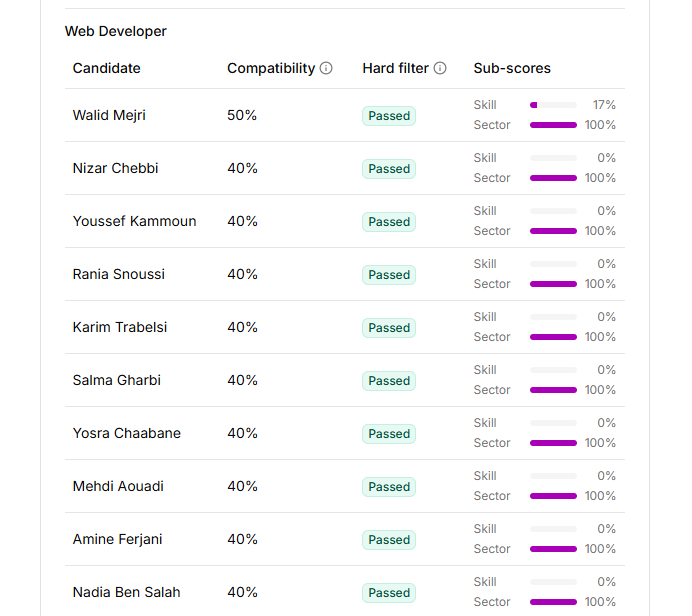
\includegraphics[width=\textwidth]{matching-hard-passed-web-dev.png}
    \caption{Web Developer: all passed}
    \label{fig:matching-web-dev-passed}
  \end{subfigure}
  \hfill
  \begin{subfigure}[t]{0.48\textwidth}
    \centering
    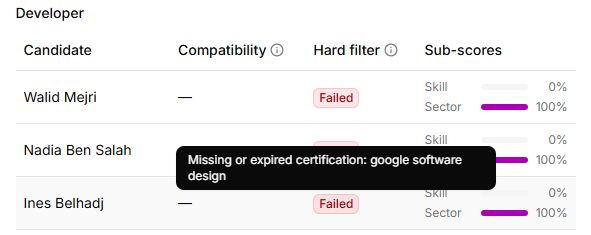
\includegraphics[width=\textwidth]{matching-dev-hard-failed-with-label-explanation.png}
    \caption{Developer: hard-filter failure}
    \label{fig:matching-dev-hard-failed}
  \end{subfigure}
  \caption[Matching results: passed vs.\ hard-filter failure]{Matching
  results, two positions: all candidates passed (left) vs.\ a hard-filter
  failure with its reason tooltip (right).}
  \label{fig:matching-results}
\end{figure}

\section{Sprint Retrospective}

\textbf{What worked:} the two-phase architecture (cheap coarse retrieval
before any expensive per-candidate work) held up under real load without
rework, and the decision to hoist position-scoped normalization/embedding
work out of the per-candidate loop during the hardening pass, rather
than deferring it as a "nice to have," turned a real
$O(\text{positions} \times \text{candidates})$ cost into
$O(\text{positions} + \text{candidates})$ before it became a problem at a
larger candidate pool.

\textbf{What didn't:} the sprint's own live-testing lesson from Sprint 1
was under-applied at first. ADQ-10 through ADQ-18 shipped and passed
their mocked tests before a single real TDR was run all the way through
the finished matching view. All four real defects in
Table~\ref{tab:s2-live-testing-defects} were sitting in code that had
been "done" for some time before live testing surfaced them. The
docker-image staleness issue
compounded this: a code fix was verified "live" twice against a
container that hadn't actually rebuilt, producing a false negative that
took real time to diagnose.

\textbf{Change for Sprint 3:} treat "demoable" and "live-tested against a
real document end to end, through a freshly rebuilt stack" as two
separate gates, not one. The first isn't sufficient evidence for the
second, and this sprint paid for conflating them.

\section{Conclusion}

Sprint 2 delivered a real, ranked, sub-scored matching pipeline running
end to end with zero LLM calls, backed by a 104-term taxonomy and an
11-candidate pool the team grew and owns itself rather than waiting on
data that was never going to arrive. Beyond the committed backlog: a
twelve-finding hardening pass fixed real correctness and efficiency
issues before they could compound in Sprint 3, and two rounds of live
testing against real TDRs found and fixed four defects no mocked test had
caught: an extraction-merge data-loss bug, a scoring-visibility gap, TDR
reprocessing accumulating stale positions indefinitely, and matching job
enqueue not resetting stale Redis progress state. Additionally, a proactive
upload-deduplication guard with an explicit \texttt{force=true} escape hatch
was added to prevent pipeline bugs from being permanently masked by file
caching. The retrieval-quality eval (Recall@3 = 1.0, Precision@3 = 0.33 across
11 varied positions) and the newly-honest gold matching set give Sprint 3's
LLM-judgment and human-in-the-loop work a real, growing foundation to build
on rather than a synthetic placeholder.
